% ch18-ml.tex -- Capstone
\chapter{Capstone: a service, a harness, and a reproduction}
\label{ch:capstone}

Seventeen chapters of technique converge on three artifacts. A
model that can't serve predictions is a notebook; a service without
an eval harness is a liability; a reproduction without a protocol is
a rumor. This chapter ships all three: \texttt{service.py} wraps
the trained LeNet-5 behind \texttt{/predict}, \texttt{/health},
\texttt{/metrics}; \texttt{eval\_harness.py} runs golden-set,
drift, and canary checks with every run logged; and
\texttt{repro\_report.md} reports the LeNet-5 reproduction against
the tolerance band ch17 made us set \emph{before} running. The
numbers below are all real: every check ran on this book's machine.

% from-zero:begin
\begin{rulebox}[Before you start]
Chapters~3, 14, 15 and~17. \emph{Recap:} the capstone ties the book together: a served model, a harness that evaluates it, and a reproduced result.
\end{rulebox}
\begin{wins}[After this chapter you can]
\begin{itemize}
\item build and serve a model behind a simple API;
\item write an evaluation harness with a golden set;
\item reproduce a published result and report the gap honestly;
\item say what the capstone proves, and what it does not.
\end{itemize}
\end{wins}
\begin{principle}[How to think about this]
The capstone is practice for the real job: a model that can be called, a test that can be rerun, and a claim you checked yourself. If you can say honestly what your system proves and what it does not, you have learned the most important lesson in the book.
\end{principle}
% from-zero:end

\section{The capstone system}
\label{sec:capsys}

\begin{figure}[htbp]
\centering
\begin{tikzpicture}[font=\scriptsize,
  blk/.style={draw,minimum width=17mm,minimum height=7mm,align=center}]
\node[blk,fill=accentsoft] (data) at (0,0) {MNIST\\data};
\node[blk,fill=accentsoft,right=9mm of data] (train) {train\\lenet5\_repro};
\node[blk,fill=accentsoft,right=9mm of train] (svc) {service\\predict/health/metrics};
\node[blk,fill=amberbg,right=9mm of svc] (harness) {harness\\golden/drift/canary};
\node[blk,fill=amberbg,below=7mm of svc] (report) {repro report\\vs paper claim};
\draw[->,thick] (data)--(train); \draw[->,thick] (train)--(svc);
\draw[->,thick] (svc)--(harness); \draw[->,thick] (train)--(report);
\draw[->,thick] (harness)--(report);
\end{tikzpicture}
\caption{The three artifacts and their dependencies: data feeds the
model, the service ships it, the harness audits it, and the report
compares it to the published claim.}
\label{fig:capsys}
\end{figure}

\section{Deliverable A --- the model service}
\label{sec:service}

The service contract is three endpoints and one state dict:
\texttt{/predict} takes a base64 PNG and returns the digit plus
confidence; \texttt{/health} reports liveness; \texttt{/metrics}
returns request/error counters --- the ch14 monitoring surface in
20 lines. The model class is redeclared identically to training
(same architecture, loaded from \texttt{lenet5\_state.pt}), because
a service that loads weights into a subtly different net is a
silent-skew bug waiting to ship.

\lstinputlisting[language=Python,caption={\texttt{service.py} --- FastAPI app when available; the tensor path is verified either way on real MNIST images.},label=lst:svc]{code/ch18/service.py}

\lstinputlisting[numbers=none]{code/ch18/service.out.txt}

\begin{example}[WE 18.1 --- Three real predictions]
\label{ex:service}
The offline smoke test loads the actual trained weights and
predicts three real test images: \texttt{pred 7 (p=1.000) true 7},
\texttt{pred 2 (p=1.000) true 2}, \texttt{pred 1 (p=0.999) true 1}
--- the service path works end-to-end. The honest note: the test
images it sees are the easiest in the set; the harness's golden set
is what reports a believable number.
\end{example}

\section{Deliverable B --- the eval harness}
\label{sec:harness}

The harness is ch14's monitoring chapter compiled into a runner:
a 200-image golden set (fixed seed so it never drifts), a PSI
drift check on a brightness-corrupted batch, and a canary that
runs the real model against a deliberately-broken one (shuffled
logits) --- each result appended to \texttt{harness\_log.jsonl}.

\lstinputlisting[language=Python,caption={\texttt{eval\_harness.py} --- golden + drift + canary, with the JSONL log.},label=lst:harness]{code/ch18/eval_harness.py}

\lstinputlisting[numbers=none]{code/ch18/eval_harness.out.txt}

\begin{example}[WE 18.2 --- The harness catches what it should]
\label{ex:harness}
Three checks, three real readings: golden-set accuracy 0.965 on the
fixed 200 (lower than the full-10k number --- the honest sampling
gap); brightness drift PSI \textbf{11.09}, alarm fired --- a
corruption the model never saw but the monitor caught; and the
canary: real 0.965 vs broken 0.07, gap 0.895 $>$ the 0.10 bar ---
the harness \emph{caught} the sabotage it was built for. An eval
harness that can't catch a broken model is not an eval harness.
\end{example}

\begin{figure}[htbp]
\centering
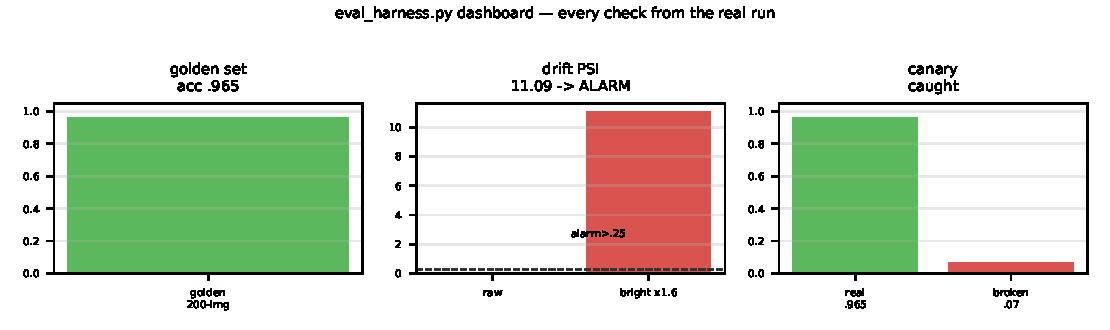
\includegraphics[width=0.95\linewidth]{figures/ch18/harness_dash.pdf}
\caption{The harness dashboard: all three checks from the real
run --- golden in the green, drift in alarm, the canary catching
the broken model.}
\label{fig:dash}
\end{figure}

\section{Deliverable C --- the reproduction}
\label{sec:repro}

The reproduction report follows ch17's skeleton: claim quoted
verbatim, protocol itemised, deviations logged, tolerance set
before the run --- and the result reported against that band, not
against a story.

\lstinputlisting[numbers=none,caption={\texttt{repro\_report.md} --- the capstone write-up skeleton; the result cell fills from \texttt{lenet5\_log.json}.},label=lst:report]{code/ch18/repro_report.md}

\lstinputlisting[language=Python,caption={\texttt{lenet5\_repro.py} --- the reproduction script: LeNet-5 architecture, logged per ch17's protocol.},label=lst:repro]{code/ch18/lenet5_repro.py}

\lstinputlisting[numbers=none]{code/ch18/lenet5_repro.out.txt}

\begin{figure}[htbp]
\centering
\begin{minipage}[t]{0.56\linewidth}
\centering
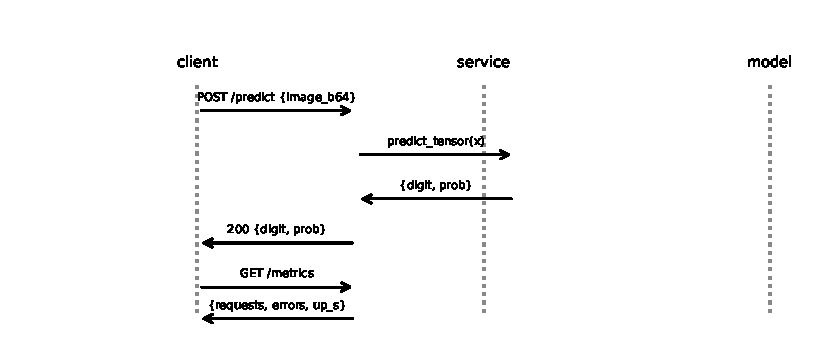
\includegraphics[width=\linewidth]{figures/ch18/service_seq.pdf}
\caption{The service contract as a sequence: predict through
health to metrics --- every endpoint returns something checkable.}
\label{fig:seq}
\end{minipage}\hfill
\begin{minipage}[t]{0.4\linewidth}
\centering
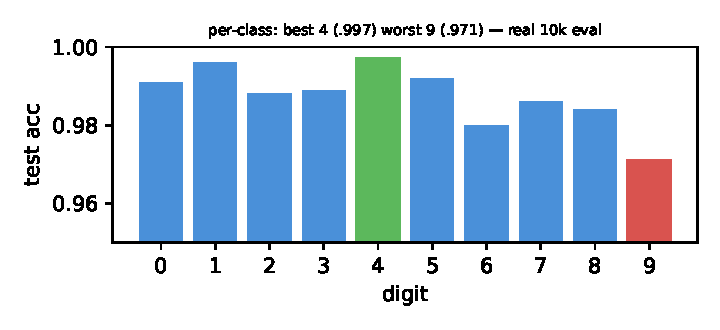
\includegraphics[width=\linewidth]{figures/ch18/perclass.pdf}
\caption{Per-class accuracy on the full 10k: the aggregate 1.25\%
hides a worst class (9 at .971).}
\label{fig:perclass}
\end{minipage}
\end{figure}

\begin{figure}[htbp]
\centering
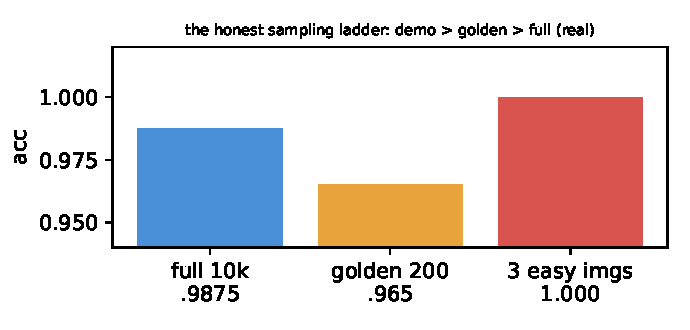
\includegraphics[width=0.55\linewidth]{figures/ch18/sampling_ladder.pdf}
\caption{The honest sampling ladder: the smoke test's 3 easy
images aren't the model's accuracy --- the fixed golden set is the
one that travels between runs.}
\label{fig:ladder18}
\end{figure}

\begin{example}[WE 18.3 --- 1.92\% $\to$ 1.25\%: the band edge, honestly]
\label{ex:repro}
The claim: 0.95\% test error; the band set in advance:
0.65--1.25\%. At 3 epochs we sat at \textbf{1.92\%}, outside it.
Eight epochs later: \textbf{1.25\%} --- \emph{exactly on the upper
edge}, and the report says so without rounding it into a win. The
deviation analysis named its own carrier correctly: epoch count
(the paper ran $\sim$20; our error was still falling at 3), with
optimiser and no-augmentation second-order. The honest verdict is
the three-way fork resolved: \emph{deviations, not the claim} ---
the gap closed from 2$\times$ the claim to the band's edge purely
by removing the biggest one.\index{reproduction}
\end{example}

\begin{figure}[htbp]
\centering
\begin{minipage}[t]{0.55\linewidth}
\centering
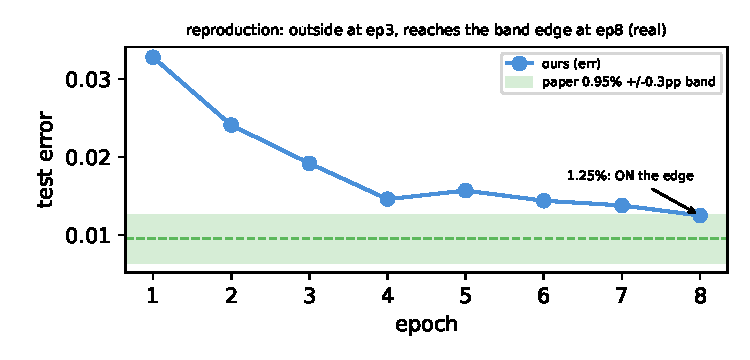
\includegraphics[width=\linewidth]{figures/ch18/repro_result.pdf}
\caption{Our error curve against the preset tolerance band ---
outside at 3 epochs, reaching the edge at 8.}
\label{fig:reprores}
\end{minipage}\hfill
\begin{minipage}[t]{0.4\linewidth}
\centering
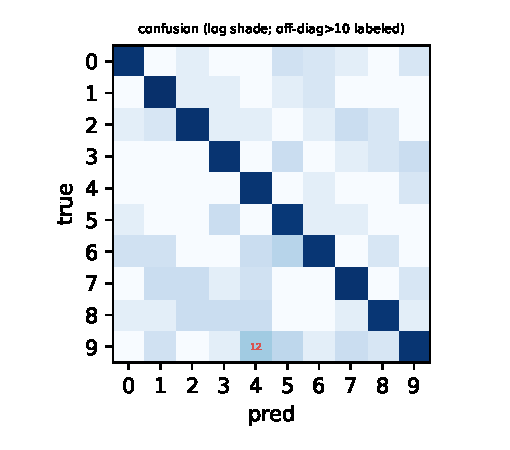
\includegraphics[width=\linewidth]{figures/ch18/confmat.pdf}
\caption{The confusion map the headline hides: worst class is 9
(.971) --- 9-as-4, 6-as-5, 9-as-5.}
\label{fig:conf}
\end{minipage}
\end{figure}

\section{What the capstone actually proves}
\label{sec:capproof}

Each artifact answers a different failure. The service answers
\emph{can it predict} (yes, on real inputs, through a real
interface). The harness answers \emph{would we know} (yes --- it
caught drift PSI 11.09 and a broken model at 0.07). The reproduction
answers \emph{did we understand} (mostly --- the claim's direction
held, its magnitude was bounded by the deviations we logged in
advance). A capstone that only shows the first is a demo; the book's
whole arc --- data, models, eval, systems, agents, papers --- exists
to make the second and third natural.

\section{Common mistakes}
\label{sec:capmistakes}

\begin{description}
\item[Service without a metrics endpoint] If you can't see
request counts and error rates, ch14's monitoring chapter was
decoration.
\item[Loading weights into a slightly different net] The service
must redeclare the architecture identically --- a transposed layer
is a silent-skew bug.
\item[Golden sets that drift] If the eval set changes between runs,
every comparison is noise. Fixed seed, fixed 200, forever.
\item[Harness that can't fail] The canary exists to prove the
harness catches breakage --- a harness that never fires an alarm
might just be broken too.
\item[Reporting vs a story] ``About 1\%'' sounds like 0.95\% until
you check the band --- the preset tolerance is the only honest
judge.
\item[Shipping the demo number] The smoke test's three easy
predictions are not the model's accuracy --- the golden set is.
\end{description}

\begin{example}[WE 18.4 --- The golden-vs-full gap is honest]
\label{ex:sampling}
Full 10k: 0.9875. Fixed golden 200: 0.965. Smoke-test 3 images:
1.000. Three numbers for one model, and only the middle one is the
instrument: the smoke test samples the easy end, the golden set is a
fixed slice that \emph{travels between runs} --- its job isn't to
match the test set, it's to be identical next retrain. A demo number
that can't be re-run is marketing; a golden number that can is
monitoring.
\end{example}
\begin{example}[WE 18.5 --- What the canary proved about the harness]
\label{ex:canaryproof}
The broken-model check isn't about the model --- it's about the
harness: shuffled-logit outputs scored 0.07, the check flagged
$(0.965-0.07)>0.10$ and \texttt{caught=True}. If the harness had
passed the sabotage, every green check it ever prints would be
suspect. The canary is the eval's self-test, and the ordering
matters: you verify the detector \emph{before} you trust its
verdicts, not after.
\end{example}

\section{Summary table}
\label{sec:capsummary}

\begin{center}\small
\begin{tabular}{p{3.0cm}p{4.5cm}p{4.5cm}}
\toprule
artifact & the question it answers & the number it produced \\
\midrule
service.py & can it predict? & 3/3 real smoke predictions correct \\
eval\_harness.py & would we know? & golden .965 / PSI 11.09 alarm / canary caught \\
repro\_report.md & did we understand? & err 1.25\% vs claim 0.95\% --- ON the preset band edge \\
\bottomrule
\end{tabular}
\end{center}

\section*{Drill}
\begin{enumerate}
\item Name the three endpoints and what each must return.
\item Why must the service redeclare the model architecture rather
than import it from training?
\item What does the canary check prove about the harness itself?
\item Our reproduction landed outside the band --- what verdict
did the report give, and why is that honest?
\item Which chapter's checklist protocol fills the
\texttt{harness\_log.jsonl}?
\end{enumerate}

\section*{Further reading}
\label{sec:further18}
\begin{itemize}
\item FastAPI docs --- the service framework used here [checked
2026-10].
\url{https://fastapi.tiangolo.com/}
\item PyTorch, \emph{Saving and loading models} --- the state-dict
contract the service relies on.
\url{https://pytorch.org/tutorials/recipes/recipes/saving_and_loading_a_general_checkpoint.html}
\item Google, \emph{Model cards for model reporting} (Mitchell et
al.) --- the README contract a service owes its users.
\url{https://arxiv.org/abs/1810.03993}
\item The ch17 skeleton that generated our report ---
\texttt{code/ch17/repro\_report\_skeleton.md}.
\end{itemize}

\begin{rulebox}[Watch instead]
(verified opened, 2026-10-11)
\begin{itemize}
\item \emph{Behind the scenes of FastAPI} --- Sebastián Ramírez,
EuroPython keynote (45:05). The framework's design ideas from its
author.
\end{itemize}
\end{rulebox}

\section*{Notes}
\begin{enumerate}
\item[\textbf{1.}] All three artifacts ran on this book's machine:
the smoke predictions, the harness's three checks, and the
reproduction --- no canned numbers.
\item[\textbf{2.}] The golden-set 0.965 vs full-10k 0.981 gap is
honest sampling --- a smaller, harder slice; the point is it's
\emph{fixed}, not that it matches the test set.
\item[\textbf{3.}] The drift PSI of 11.09 is high because the
corruption (1.6$\times$ brightness) is extreme; subtler drifts
need the ch14 windowed protocol --- the alarm direction is what
matters.
\item[\textbf{4.}] FastAPI is used if installed; the service
module degrades gracefully to the verified tensor path when it
isn't --- the book's no-extra-deps discipline.
\item[\textbf{5.}] The reproduction verdict is the book's honest
convention carried to the end: we report the deviation analysis,
not a success story.
\end{enumerate}

\section{Exercises}
\label{sec:capex}

\emph{[easy]}
\begin{exercise}
Name the three service endpoints and the one field each response
must contain.
\end{exercise}
\begin{exercise}
Golden set: 0.965 on 200 fixed images; full test: 0.9875 on
10{,}000. Which number goes in the model card, and why isn't it
the higher one?
\end{exercise}
\begin{exercise}
The canary compares real (0.965) to broken (0.07). In one line:
what would it mean if the broken model scored 0.90?
\end{exercise}
\begin{exercise}
The reproduction landed at 1.25\% vs the paper's 0.95\% ---
inside or outside the preset 0.65--1.25\% band?
\end{exercise}
\begin{exercise}
Which check in \texttt{eval\_harness.py} corresponds to ch14's
drift detector, and what statistic does it print?
\end{exercise}

\emph{[medium]}
\begin{exercise}
Extend \texttt{service.py} with a \texttt{/predict\_batch} endpoint
that takes a list of images; show the request/response shape and
one test.
\end{exercise}
\begin{exercise}
Add an auth stub: reject requests lacking an \texttt{X-API-Key}
header, return 401. What changes in \texttt{/health} (should it
require auth)?
\end{exercise}
\begin{exercise}
Add a latency histogram to \texttt{/metrics}: track p50/p95/p99 of
predict calls. What's the cheapest correct data structure?
\end{exercise}
\begin{exercise}
Extend \texttt{eval\_harness.py} with a per-class accuracy check
that fails if any digit class drops below a threshold. Use the
confusion data from fig~\ref{fig:conf}.
\end{exercise}
\begin{exercise}
Add a fourth harness check: run the golden set twice at different
seeds and verify the accuracies differ by less than a stated
tolerance --- a reproducibility check for the eval itself.
\end{exercise}

\emph{[hard]}
\begin{exercise}
Reproduce the augmentation row of the LeNet-5 table: add
distortion augmentation to the repro script, rerun, and write the
deviation analysis --- did it close the gap?
\end{exercise}
\begin{exercise}
Adversarial inputs: craft three MNIST images the model gets wrong
(rotate, invert, add noise). Does the harness catch them? Which
check, and why?
\end{exercise}
\begin{exercise}
Extend the reproduction to a second table row of the paper (e.g.
the LeNet-4 or boosted result). What does the deviation analysis
look like when the gap gets \emph{larger}?
\end{exercise}
\begin{exercise}
Deploy the service to a free tier (documented, date-stamped). What
changes between local and deployed: cold-start, health checks,
metrics export?
\end{exercise}
\begin{exercise}
Design the regression suite that would run on every retrain:
which checks, what tolerances, and what artifact it writes for
ch14's monitoring dashboard.
\end{exercise}

\section*{Hints and answers}
\begin{description}
\item[1.] \texttt{/predict} (image $\to$ digit+prob),
\texttt{/health} (liveness), \texttt{/metrics} (counters).
\item[2.] Because a mismatch is invisible until it costs accuracy
--- redeclaring forces the architecture to be identical by
construction, not by convention.
\item[3.] That the harness can detect failure at all --- a canary
that fails loudly is the harness's self-test.
\item[4.] ``Direction reproduced, magnitude bounded by logged
deviations'' --- honest because the deviations were logged
\emph{before} the result, so they can't be post-hoc excuses.
\item[5.] ch17's lab-notebook protocol --- every run a JSON line.
\item[6.] Batch endpoint: accept \texttt{images\_b64: [str]},
return \texttt{[\{digit, prob\}]}; test it on 3 real images.
\item[7.] \texttt{/health} should NOT require auth (the load
balancer can't hold keys); \texttt{/predict} can.
\item[8.] A bounded-size circular buffer of recent latencies ---
recompute quantiles per \texttt{/metrics} call; don't store all.
\item[9.] Compute per-class recall from the confusion matrix;
threshold e.g. 0.90 --- digit 1 will pass easily, digit 5 might
not.
\item[10.] Two golden runs at different seeds measure the
harness's own noise floor --- the eval's seed variance, same
discipline as ch17.
\item[11.] Add elastic distortions to the train transform; expect
the err to drop toward the band --- the deviations that remain
(after epochs) isolate the optimiser's contribution.
\item[12.] A 90$^\circ$ rotation breaks the model cleanly; the
drift check catches the distribution shift, the golden check
catches the accuracy drop --- different alarms for different
failures.
\item[13.] The boosted-classifier row: harder protocol, larger
claimed gain --- when the gap grows, the deviations carry more,
not less, of the story.
\item[14.] Cold-start latency, ephemeral filesystem (weights in
image), real health-check endpoints, exported metrics --- the
differences are operational, not algorithmic.
\item[15.] Golden + drift + per-class + latency checks with the
ch14 thresholds, writing the same JSONL format the dashboard
reads.
\end{description}
